% answers.tex —— 2011 年·广东卷·文科 · 参考答案与详细解析片段
% 由 tools/generate_projects.py 依来源总账自 2011/2011_数学真题_广东文_试题.md + 2011/2011_数学真题_广东文_解析正文.md + 2011/2011_数学真题_广东文_答案要点.md 生成，勿手改（改源 MD 后重跑）
\begin{gktip}
固定源 PDF 只有题面、没有答案页，原页未印分值，也未印参考公式（原页未标）。以下解析与结论均由本库独立推导（非官方答案，等级 D），并按 600 dpi 位图逐栏复核题面。本 PDF 没有文字层，\texttt{pdftotext} 取不出任何字符，题面一律以位图核对。

【源疑点】原页各题均未印分值；第 13 题所需的回归系数公式原页未给，本解析按最小二乘式自行给出。第 16 题第（2）问的「求 $\sin(\alpha+\beta)$ 的值」在原页跨两行排印，第二行只有「的值．」。第 21 题题设只要求 $\angle MPO=\angle AOP$，当 $M$ 落在射线 $OA$ 上（此时 $M$ 在 $x$ 轴负半轴、位于直线 $l$ 上）时该条件也成立，题面未把这种位置排除，本解析按通行处理只取非退化的抛物线，并在第 21 题内说明。

【图形说明】第 9、15、18 题的图形依原页拓扑重绘，不按比例。第 9 题按原页标注正视图左边 $2\sqrt3$、侧视图底边 $2$、俯视图斜边 $2$；第 18 题按原页的斜投影示意重绘，并照原页保留 $H'B'$ 直线下方那条向下微凹的虚线弧（原页如此，本库不赋新的几何含义）。原页其余各题无图。
\end{gktip}

\begin{answer}
\gksolhead{1}{}

\textbf{题目}：

设复数 $z$ 满足 $\mathrm i z=1$，其中 $\mathrm i$ 为虚数单位，则 $z=$\mbox{（　　）}

（A）$-\mathrm i$

（B）$\mathrm i$

（C）$-1$

（D）$1$

\Needspace{4\baselineskip}
\textbf{解析}
\Needspace{5\baselineskip}
方程 $\mathrm i z=1$ 是一次的，两边同乘 $-\mathrm i$ 即可（$-\mathrm i$ 是 $\mathrm i$ 的倒数，因为 $\mathrm i\cdot(-\mathrm i)=1$）：
\nopagebreak[4]
\[
z=\frac{1}{\mathrm i}=\frac{1}{\mathrm i}\cdot\frac{\mathrm i}{\mathrm i}=\frac{\mathrm i}{\mathrm i^2}=-\mathrm i.
\]
逐项排除：
\begin{itemize}
\item A $-\mathrm i$：正是所求；
\item B $\mathrm i$：$\mathrm i\cdot\mathrm i=\mathrm i^2=-1\neq1$；
\item C $-1$：$\mathrm i\cdot(-1)=-\mathrm i\neq1$；
\item D $1$：$\mathrm i\cdot1=\mathrm i\neq1$。
\end{itemize}
二次复算：把 $z=-\mathrm i$ 代回原方程，$\mathrm i\cdot(-\mathrm i)=-\mathrm i^2=-(-1)=1$，成立。
选 A。

\gkanswer{答案：A。}

\end{answer}
\begin{answer}
\gksolhead{2}{}

\textbf{题目}：

已知集合 $A=\{(x,y)\mid x,y\text{ \text{为实数，且} }x^2+y^2=1\}$，$B=\{(x,y)\mid x,y\text{ \text{为实数，且} }x+y=1\}$，则 $A\cap B$ 的元素个数为\mbox{（　　）}

（A）$4$

（B）$3$

（C）$2$

（D）$1$

\Needspace{4\baselineskip}
\textbf{解析}
\Needspace{5\baselineskip}
$A$ 是单位圆 $x^2+y^2=1$ 上全体点构成的集合，$B$ 是直线 $x+y=1$ 上全体点构成的集合，所以 $A\cap B$ 就是圆与直线的公共点集，元素个数等于交点个数。把 $y=1-x$ 代入：
\nopagebreak[4]
\[
x^2+(1-x)^2=1\ \Longrightarrow\ 2x^2-2x+1=1\ \Longrightarrow\ 2x(x-1)=0,
\]
得 $x=0$ 或 $x=1$，对应点 $(0,1)$ 与 $(1,0)$，共 $2$ 个。
逐项排除：
\begin{itemize}
\item A $4$：圆与直线最多 $2$ 个公共点，不可能有 $4$ 个；
\item B $3$：同上，一次方程与二次方程联立不可能给出 $3$ 个解；
\item C $2$：与计算结果相符；
\item D $1$：这相当于认为直线与圆相切。圆心 $(0,0)$ 到 $x+y=1$ 的距离是 $\dfrac{1}{\sqrt2}<1$，直线与圆相交于两点，不是相切。
\end{itemize}
二次复算：$(0,1)$ 满足 $0^2+1^2=1$ 且 $0+1=1$；$(1,0)$ 满足 $1^2+0^2=1$ 且 $1+0=1$。两点互异，故恰为 $2$ 个。
选 C。

\gkanswer{答案：C。}

\end{answer}
\begin{answer}
\gksolhead{3}{}

\textbf{题目}：

已知向量 $\boldsymbol a=(1,2)$，$\boldsymbol b=(1,0)$，$\boldsymbol c=(3,4)$．若 $\lambda$ 为实数，$(\boldsymbol a+\lambda\boldsymbol b)\parallel\boldsymbol c$，则 $\lambda=$\mbox{（　　）}

（A）$\frac14$

（B）$\frac12$

（C）$1$

（D）$2$

\Needspace{4\baselineskip}
\textbf{解析}
\Needspace{5\baselineskip}
先算出和向量：
\nopagebreak[4]
\[
\boldsymbol a+\lambda\boldsymbol b=(1,2)+\lambda(1,0)=(1+\lambda,\,2).
\]
\Needspace{5\baselineskip}
两向量平行，等价于对应分量成比例（$\boldsymbol c=(3,4)$ 的两个分量都不为零）：
\nopagebreak[4]
\[
\frac{1+\lambda}{3}=\frac{2}{4}=\frac12\ \Longrightarrow\ 1+\lambda=\frac32\ \Longrightarrow\ \lambda=\frac12.
\]
逐项排除：
\begin{itemize}
\item A $\lambda=\dfrac14$：$\boldsymbol a+\lambda\boldsymbol b=\left(\dfrac54,2\right)$，比例 $\dfrac{5/4}{3}=\dfrac{5}{12}\neq\dfrac12$，不平行；
\item B $\lambda=\dfrac12$：与计算结果相同；
\item C $\lambda=1$：得 $(2,2)$，比例 $\dfrac23\neq\dfrac12$，不平行（它平行于 $(1,1)$）；
\item D $\lambda=2$：得 $(3,2)$，第一分量对上了而第二分量应为 $4$，不平行。
\end{itemize}
二次复算：$\lambda=\dfrac12$ 时 $\boldsymbol a+\lambda\boldsymbol b=\left(\dfrac32,2\right)=\dfrac12(3,4)=\dfrac12\boldsymbol c$，确实是 $\boldsymbol c$ 的倍数。
选 B。

\gkanswer{答案：B。}

\end{answer}
\begin{answer}
\gksolhead{4}{}

\textbf{题目}：

函数 $f(x)=\dfrac{1}{1-x}+\lg(1+x)$ 的定义域是\mbox{（　　）}

（A）$(-\infty,-1)$

（B）$(1,+\infty)$

（C）$(-1,1)\cup(1,+\infty)$

（D）$(-\infty,+\infty)$

\Needspace{4\baselineskip}
\textbf{解析}
定义域要两个条件同时成立：
\begin{itemize}
\item 分式的分母不为零：$1-x\neq0$，即 $x\neq1$；
\item 对数的真数为正：$1+x>0$，即 $x>-1$。
\end{itemize}

两者取交得 $x>-1$ 且 $x\neq1$，即 $(-1,1)\cup(1,+\infty)$。
逐项排除：
\begin{itemize}
\item A $(-\infty,-1)$：这一段使 $1+x<0$，对数无意义；
\item B $(1,+\infty)$：漏掉了 $(-1,1)$ 这一段；
\item C $(-1,1)\cup(1,+\infty)$：与计算结果相符；
\item D $(-\infty,+\infty)$：$x=1$ 使分母为零、$x=-2$ 使真数为负，都不在定义域内。
\end{itemize}
二次复算：取 $x=0$，$f(0)=\dfrac{1}{1}+\lg1=1$，有意义；取 $x=1$，分母为零，无意义；取 $x=-1$，真数为零，无意义；取 $x=-2$，真数为 $-1$，无意义。与所得区间一致。
选 C。

\gkanswer{答案：C。}

\end{answer}
\begin{answer}
\gksolhead{5}{}

\textbf{题目}：

不等式 $2x^2-x-1>0$ 的解集是\mbox{（　　）}

（A）$\left(-\frac12,1\right)$

（B）$(1,+\infty)$

（C）$(-\infty,1)\cup(2,+\infty)$

（D）$\left(-\infty,-\frac12\right)\cup(1,+\infty)$

\Needspace{4\baselineskip}
\textbf{解析}
\Needspace{5\baselineskip}
先因式分解：
\nopagebreak[4]
\[
2x^2-x-1=(2x+1)(x-1),
\]
\Needspace{5\baselineskip}
对应方程的两根是 $x=-\dfrac12$ 与 $x=1$。二次项系数 $2>0$，抛物线开口向上，故不等式 $>0$ 的解集是两根之外：
\nopagebreak[4]
\[
\left(-\infty,-\frac12\right)\cup(1,+\infty).
\]
逐项排除：
\begin{itemize}
\item A $\left(-\dfrac12,1\right)$：这恰是 $2x^2-x-1<0$ 的解集，方向相反；
\item B $(1,+\infty)$：漏掉左支 $\left(-\infty,-\dfrac12\right)$；
\item C $(-\infty,1)\cup(2,+\infty)$：端点 $2$ 不是根。取 $x=0\in(-\infty,1)$，左边为 $-1<0$，可见该区间混入了不合的点；
\item D $\left(-\infty,-\dfrac12\right)\cup(1,+\infty)$：与计算结果相符。
\end{itemize}
二次复算：取 $x=-1$（在左支），$2+1-1=2>0$，成立；取 $x=2$（在右支），$8-2-1=5>0$，成立；取 $x=0$（在两根之间），$-1>0$ 不成立。
选 D。

\gkanswer{答案：D。}

\end{answer}
\begin{answer}
\gksolhead{6}{}

\textbf{题目}：

\Needspace{5\baselineskip}
已知平面直角坐标系 $xOy$ 上的区域 $D$ 由不等式组
\nopagebreak[4]
\[
\begin{cases}
0\leqslant x\leqslant\sqrt2,\\
y\leqslant2,\\
x\leqslant\sqrt2y
\end{cases}
\]
给定．若 $M(x,y)$ 为 $D$ 上的动点，点 $A$ 的坐标为 $(\sqrt2,1)$，则 $z=\overrightarrow{OM}\cdot\overrightarrow{OA}$ 的最大值为\mbox{（　　）}

（A）$3$

（B）$4$

（C）$3\sqrt2$

（D）$4\sqrt2$

\Needspace{4\baselineskip}
\textbf{解析}
\Needspace{5\baselineskip}
先画出可行域。三条边界是 $x=0$、$x=\sqrt2$、$y=2$ 与直线 $x=\sqrt2y$（即 $y=\dfrac{x}{\sqrt2}$）。由 $0\leqslant x\leqslant\sqrt2$ 与 $y\geqslant\dfrac{x}{\sqrt2}$ 得 $y\geqslant0$，与 $y\leqslant2$ 合起来，$D$ 是由四个顶点
\nopagebreak[4]
\[
(0,0),\qquad(\sqrt2,1),\qquad(\sqrt2,2),\qquad(0,2)
\]
围成的四边形（含边界）。
\Needspace{5\baselineskip}
目标函数是数量积：
\nopagebreak[4]
\[
z=\overrightarrow{OM}\cdot\overrightarrow{OA}=x\cdot\sqrt2+y\cdot1=\sqrt2x+y.
\]
\Needspace{5\baselineskip}
$z$ 关于 $(x,y)$ 是线性的，最值必在顶点处取得：
\nopagebreak[4]
\[
z(0,0)=0,\qquad z(\sqrt2,1)=2+1=3,\qquad z(\sqrt2,2)=2+2=4,\qquad z(0,2)=2.
\]
故最大值为 $4$。
逐项排除：
\begin{itemize}
\item A $3$：这是顶点 $(\sqrt2,1)$ 处的值，不是最大值；
\item B $4$：与计算结果相符；
\item C $3\sqrt2$：任何顶点处的 $z$ 值都不是 $3\sqrt2\approx4.24$；
\item D $4\sqrt2$：$z$ 在 $D$ 上的最大值不超过 $\sqrt2\cdot\sqrt2+2=4$，而 $4\sqrt2\approx5.66>4$，不可能取到。
\end{itemize}
二次复算（沿四条边逐段检验）：在 $y=\dfrac x{\sqrt2}$（$0\leqslant x\leqslant\sqrt2$）上 $z=\sqrt2x+\dfrac x{\sqrt2}=\dfrac{3x}{\sqrt2}\in[0,3]$；在 $x=\sqrt2$（$1\leqslant y\leqslant2$）上 $z=2+y\in[3,4]$；在 $y=2$（$0\leqslant x\leqslant\sqrt2$）上 $z=\sqrt2x+2\in[2,4]$；在 $x=0$（$0\leqslant y\leqslant2$）上 $z=y\in[0,2]$。四段的并集为 $[0,4]$，最大值确为 $4$。
选 B。

\gkanswer{答案：B。}

\end{answer}
\begin{answer}
\gksolhead{7}{}

\textbf{题目}：

正五棱柱中，不同在任何侧面且不同在任何底面的两顶点的连线称为它的对角线，那么一个正五棱柱对角线的条数共有\mbox{（　　）}

（A）$20$

（B）$15$

（C）$12$

（D）$10$

\Needspace{4\baselineskip}
\textbf{解析}
把正五棱柱的十个顶点分成上下两层：上底 $a_1,a_2,\dots,a_5$，下底 $b_1,b_2,\dots,b_5$，其中 $a_i$ 在 $b_i$ 的正上方（下标按模 $5$ 计算）。题目把对角线定义为「不同在任何侧面且不同在任何底面的两顶点连线」，因此只需数跨层的连线 $a_ib_j$。
\begin{itemize}
\item 跨层连线共 $5\times5=25$ 对；
\item 若 $j\equiv i\pmod5$，两点在同一条竖直棱上，同处两个侧面，不是对角线（$5$ 对）；
\item 若 $j\equiv i\pm1\pmod5$，两点同处一个侧面 $a_ia_{i\pm1}b_{i\pm1}b_i$，也不是对角线（每点 $2$ 对，共 $10$ 对）。
\end{itemize}

每点剩下 $5-1-2=2$ 个可用点，合计 $5\times2=10$ 条。
逐项排除：
\begin{itemize}
\item A $20$：等于 $25-5$，只扣掉了同一条竖直棱上的 $5$ 对，漏掉同处一个侧面的另外 $10$ 条侧面对角线；
\item B $15$：等于 $25-10$，只扣掉了 $10$ 条侧面对角线，漏掉 $5$ 条竖直棱；
\item C $12$：在正确的 $10$ 条之外多出 $2$ 条，恰好是把某一个侧面上的 $2$ 条对角线也当成了对角线；
\item D $10$：与计算结果相符。
\end{itemize}
二次复算（用总条数倒扣）：十个顶点两两连线共 $\mathrm C_{10}^2=45$ 条；减去同一底面上的连线 $2\mathrm C_5^2=20$ 条，得 $25$ 条跨层连线；再减去同处一个侧面的 $5$ 条竖直棱与 $10$ 条侧面对角线，余 $25-5-10=10$ 条。
选 D。

\gkanswer{答案：D。}

\end{answer}
\begin{answer}
\gksolhead{8}{}

\textbf{题目}：

设圆 $C$ 与圆 $x^2+(y-3)^2=1$ 外切，且与直线 $y=0$ 相切，则 $C$ 的圆心轨迹为\mbox{（　　）}

（A）抛物线

（B）双曲线

（C）椭圆

（D）圆

\Needspace{4\baselineskip}
\textbf{解析}
设圆 $C$ 的圆心为 $(a,b)$、半径为 $r>0$。已知圆 $x^2+(y-3)^2=1$ 的圆心为 $(0,3)$、半径为 $1$。
\Needspace{5\baselineskip}
「与直线 $y=0$ 相切」给出 $r=|b|$；「与已知圆外切」给出圆心距等于半径之和：
\nopagebreak[4]
\[
\sqrt{a^2+(b-3)^2}=|b|+1.
\]
分两种情形：
\begin{itemize}
\item 若 $b>0$，则 $|b|=b$，两边平方：$a^2+b^2-6b+9=b^2+2b+1$，化简得 $a^2=8b-8$，即
\end{itemize}
\nopagebreak[4]
\[
b=\frac{a^2}{8}+1,
\]
这是开口向上的抛物线；
\begin{itemize}
\item 若 $b<0$，则 $|b|=-b$，右边为 $1-b$。平方得 $a^2+b^2-6b+9=b^2-2b+1$，化简得 $a^2=4b-8$，右端小于 $-8$，无解（几何上：圆心在 $x$ 轴下方时，它与 $y=0$ 相切且与位于上方的已知圆外切，圆心距必大于两者半径之和）。
\end{itemize}

故圆心轨迹是抛物线 $b=\dfrac{a^2}{8}+1$，即 $x^2=8(y-1)$。
逐项排除：
\begin{itemize}
\item A 抛物线：与上面的一次—二次关系相符；
\item B 双曲线：双曲线要求平方项系数异号，上式只有一个平方项；
\item C 椭圆：椭圆要求两个平方项系数同号且都不为零，上式没有 $b^2$ 项；
\item D 圆：圆要求 $a^2$ 与 $b^2$ 项系数相等，上式没有 $b^2$ 项。
\end{itemize}
二次复算：取 $a=0$，得 $b=1$，此时 $C:x^2+(y-1)^2=1$，与已知圆的圆心距为 $2=1+1$（外切），与 $y=0$ 也相切，符合；再取 $a=4$，得 $b=3$，半径 $r=3$，与已知圆的圆心距 $\sqrt{16+0}=4=3+1$，也外切，符合。
选 A。

\gkanswer{答案：A。}

\end{answer}
\begin{answer}
\gksolhead{9}{}

\textbf{题目}：

如图，某几何体的正视图（主视图），侧视图（左视图）和俯视图分别是等边三角形，等腰三角形和菱形，则该几何体的体积为\mbox{（　　）}

（A）$4\sqrt3$

（B）$4$

（C）$2\sqrt3$

（D）$2$
\nopagebreak[4]
\begin{center}% 2011 年广东卷文科第 9 题：由三视图求几何体体积。
% 来源 PDF：普通高考/2011/2011广东文.pdf，SHA-256 b42cd0aaa193fefb6dcb39d1ae186d536a83fafbd4a64975deafbea5613d98ce。
% 原页：第 1 页（A3 三栏）第 2 栏上部，书页码 665。
% 重绘依据：照原页——左上为正（主）视图，等边三角形，左右两顶点分别引出尺寸界线，
%   沿左边外侧以双向箭头标注 2√3；三角形内有一条从顶点到底边中点的竖直线。
%   右上为侧（左）视图，等腰三角形，底边中线向两侧各画一段带箭头的尺寸线，数字 2 落在两箭头之间；
%   三角形内同样有一条竖直线。左下为俯视图，菱形，两条对角线都画出，左上斜边外侧以双向箭头标注 2。
%   三视图下各标名称；原页不画顶点圆点、不标其余尺寸。本图按原页拓扑与标注重绘，不按比例。
\begin{tikzpicture}[scale=0.82, >=stealth, semithick]
  \coordinate (P) at (1.7321,3);
  \coordinate (L) at (0,0);
  \coordinate (R) at (3.4641,0);
  % 正（主）视图：正三角形，顶点到底边中点的竖直线
  \draw (L) -- (R) -- (P) -- cycle;
  \draw (P) -- (1.7321,0);
  % 左边外侧的尺寸界线与尺寸线，标注 2√3
  \draw (L) -- (-0.433,0.25);
  \draw (P) -- (1.299,3.25);
  \draw[<->] (-0.433,0.25) -- (1.299,3.25);
  \node[rotate=60, fill=white, inner sep=1pt] at (0.15,1.98) {$2\sqrt3$};
  \node at (1.7321,-0.72) {正视图};
  % 侧（左）视图：底边 2、高 3 的等腰三角形，含竖直线
  \draw (5.2,0) -- (7.2,0) -- (6.2,3) -- cycle;
  \draw (6.2,3) -- (6.2,0);
  \draw[<->] (5.2,-0.45) -- (5.89,-0.45);
  \draw[<->] (6.51,-0.45) -- (7.2,-0.45);
  \node at (6.2,-0.45) {$2$};
  \draw (5.2,0) -- (5.2,-0.45);
  \draw (7.2,0) -- (7.2,-0.45);
  \node at (6.2,-1.12) {侧视图};
  % 俯视图：对角线 2√3（水平）与 2（竖直）的菱形，两条对角线都画出
  \draw (0,-2.2) -- (1.7321,-1.2) -- (3.4641,-2.2) -- (1.7321,-3.2) -- cycle;
  \draw (0,-2.2) -- (3.4641,-2.2);
  \draw (1.7321,-1.2) -- (1.7321,-3.2);
  % 左上斜边外侧的尺寸界线与尺寸线，标注 2（尺寸线平行于该边、向外侧偏移）
  \draw (0,-2.2) -- (-0.25,-1.767);
  \draw (1.7321,-1.2) -- (1.482,-0.767);
  \draw[<->] (-0.25,-1.767) -- (1.482,-0.767);
  \node[rotate=30, fill=white, inner sep=1pt] at (0.30,-1.55) {$2$};
  \node at (1.7321,-3.88) {俯视图};
\end{tikzpicture}
\end{center}
\nopagebreak[4]
\Needspace{4\baselineskip}
\textbf{解析}
先由三视图定形。俯视图是菱形，故底面为菱形，其两条对角线分别是正视图、侧视图中三角形的底边；正视图、侧视图都是三角形，说明几何体是顶点在底面中心正上方的四棱锥。
\begin{itemize}
\item 正视图：等边三角形，左边标注 $2\sqrt3$（原页尺寸线沿左边），故其边长 $2\sqrt3$；三角形的底边是底面菱形的长对角线 $2\sqrt3$，两腰是锥顶到长对角线两端点的棱的投影，长 $\sqrt{h^2+\left(\sqrt3\right)^2}=2\sqrt3$，解得高 $h=3$；
\item 侧视图：等腰三角形，底边标注 $2$（底面菱形的短对角线），两条腰是顶点到短对角线两端点的棱的投影，长 $\sqrt{h^2+1^2}=\sqrt{10}$，不是等边三角形，恰与「等腰」相符；
\item 俯视图：菱形边长标注 $2$，与 $\sqrt{\left(\sqrt3\right)^2+1^2}=2$ 相符，验证了上述两条对角线。
\end{itemize}

\Needspace{5\baselineskip}
底面积与体积：
\nopagebreak[4]
\[
S=\frac12\times2\sqrt3\times2=2\sqrt3,\qquad
V=\frac13Sh=\frac13\times2\sqrt3\times3=2\sqrt3.
\]
逐项排除：
\begin{itemize}
\item A $4\sqrt3$：相当于把系数 $\dfrac13$ 误成 $\dfrac23$（$\dfrac23\times2\sqrt3\times3=4\sqrt3$）；
\item B $4$：把菱形面积按矩形 $2\times2=4$ 计，忽略了菱形只占外接矩形的一半（$\dfrac13\times4\times3=4$）；
\item C $2\sqrt3$：与计算结果相符；
\item D $2$：把底面积误算成 $\dfrac12\times2\times2=2$，漏掉了长对角线上的 $\sqrt3$。
\end{itemize}
二次复算（坐标法）：以菱形中心为原点、两条对角线为坐标轴，底面四顶点为 $(\pm\sqrt3,0,0)$、$(0,\pm1,0)$，锥顶为 $(0,0,3)$。到长对角线两端点的棱长 $\sqrt{3+0+9}=2\sqrt3$，正是正视图的边长；到短对角线两端点的棱长 $\sqrt{0+1+9}=\sqrt{10}$，正是侧视图的腰长；两者都与原页图形一致。体积 $V=\dfrac13\times2\sqrt3\times3=2\sqrt3$，与上面一致。
选 C。

\gkanswer{答案：C。}

\end{answer}
\begin{answer}
\gksolhead{10}{}

\textbf{题目}：

设 $f(x)$，$g(x)$，$h(x)$ 是 $\mathbf R$ 上的任意实值函数．如下定义两个函数 $(f\circ g)(x)$ 和 $(f\bullet g)(x)$：对任意 $x\in\mathbf R$，$(f\circ g)(x)=f(g(x))$；$(f\bullet g)(x)=f(x)g(x)$，则下列等式恒成立的是\mbox{（　　）}

（A）$((f\circ g)\bullet h)(x)=((f\bullet h)\circ(g\bullet h))(x)$

（B）$((f\bullet g)\circ h)(x)=((f\circ h)\bullet(g\circ h))(x)$

（C）$((f\circ g)\circ h)(x)=((f\circ h)\circ(g\circ h))(x)$

（D）$((f\bullet g)\bullet h)(x)=((f\bullet h)\bullet(g\bullet h))(x)$

\Needspace{4\baselineskip}
\textbf{解析}
关键是两条定义的差别：$\circ$ 是复合（先内后外），$\bullet$ 是逐点相乘。按定义把 A 的两边分别展开，左边为 $\left((f\circ g)\bullet h\right)(x)=(f\circ g)(x)\cdot h(x)=f\big(g(x)\big)h(x)$，右边为 $\big((f\bullet h)\circ(g\bullet h)\big)(x)=(f\bullet h)\big((g\bullet h)(x)\big)=f\big(g(x)h(x)\big)\cdot h\big(g(x)h(x)\big)$，一般不等于 $f\big(g(x)\big)h(x)$。
逐项验证（取 $f(x)=x$、$g(x)=x^2$、$h(x)=2$ 作反例）：
\begin{itemize}
\item A 左边 $=(f\circ g)(x)h(x)=x^2\cdot2=2x^2$；右边 $=(f\bullet h)\big((g\bullet h)(x)\big)=f(2x^2)\cdot h(2x^2)=2x^2\cdot2=4x^2$。$2x^2\neq4x^2$，不恒成立；
\item B 左边 $=\big((f\bullet g)\circ h\big)(x)=(f\bullet g)\big(h(x)\big)=f(2)g(2)=2\cdot4=8$；右边 $=\big((f\circ h)\bullet(g\circ h)\big)(x)=f\big(h(x)\big)\cdot g\big(h(x)\big)=f(2)g(2)=2\cdot4=8$。两边相等。事实上对任意 $x$ 都有
\end{itemize}
\nopagebreak[4]
\[
\big((f\bullet g)\circ h\big)(x)=(f\bullet g)\big(h(x)\big)=f\big(h(x)\big)g\big(h(x)\big)=\big((f\circ h)\bullet(g\circ h)\big)(x),
\]
恒成立；
\begin{itemize}
\item C 左边 $=\big((f\circ g)\circ h\big)(x)=f\big(g(h(x))\big)=f\big(g(2)\big)=f(4)=4$；右边 $=\big((f\circ h)\circ(g\circ h)\big)(x)=(f\circ h)\big((g\circ h)(x)\big)=f\big(h(4)\big)=f(2)=2$。$4\neq2$，不恒成立；
\item D 左边 $=\big((f\bullet g)\bullet h\big)(x)=f(x)g(x)h(x)=x\cdot x^2\cdot2=2x^3$；右边 $=\big((f\bullet h)\bullet(g\bullet h)\big)(x)=(2x)(2x^2)=4x^3$。$2x^3\neq4x^3$，不恒成立。
\end{itemize}
二次复算（换一组函数）：取 $f(x)=2x$、$g(x)=x+1$、$h(x)=3$，则 B 的左边 $=(f\bullet g)\big(h(x)\big)=f(3)g(3)=6\times4=24$，右边 $=f\big(h(x)\big)g\big(h(x)\big)=f(3)g(3)=24$，仍相等；A 的左边 $=f\big(g(x)\big)h(x)=2(x+1)\cdot3=6x+6$，右边 $=f\big(g(x)h(x)\big)h\big(g(x)h(x)\big)=2\cdot3(x+1)\cdot3=18x+18$，仍不等。
选 B。

\gkanswer{答案：B。}

\end{answer}
\begin{answer}
\gksolhead{11}{}

\textbf{题目}：

已知 $\{a_n\}$ 是递增的等比数列，$a_2=2$，$a_4-a_3=4$，则此数列的公比 $q=$ \gkblank{}。

\Needspace{4\baselineskip}
\textbf{解析}
\Needspace{5\baselineskip}
设公比为 $q$。由 $a_2=2$ 得 $a_3=a_2q=2q$、$a_4=a_2q^2=2q^2$，代入 $a_4-a_3=4$：
\nopagebreak[4]
\[
2q^2-2q=4\ \Longrightarrow\ q^2-q-2=0\ \Longrightarrow\ (q-2)(q+1)=0,
\]
得 $q=2$ 或 $q=-1$。
题设「$\{a_n\}$ 是递增的等比数列」，要求 $q>0$（且首项为正时 $0<q<1$ 会递减，$q>1$ 才递增；此处 $a_2=2>0$，故 $q>1$）。$q=-1$ 给出摆动数列 $-2,2,-2,2,\cdots$，不递增，舍去；$q=2$ 给出 $1,2,4,8,\cdots$，递增。
代回验证：$q=2$、$a_2=2$ 时 $a_3=4$、$a_4=8$，$a_4-a_3=4$，且数列递增，两个条件都满足。

\gkanswer{答案：$2$。}

\end{answer}
\begin{answer}
\gksolhead{12}{}

\textbf{题目}：

设函数 $f(x)=x^3\cos x+1$．若 $f(a)=11$，则 $f(-a)=$ \gkblank{}。

\Needspace{4\baselineskip}
\textbf{解析}
\Needspace{5\baselineskip}
把 $f(x)$ 拆成一个奇函数加一个常数。令 $g(x)=x^3\cos x$，则
\nopagebreak[4]
\[
g(-x)=(-x)^3\cos(-x)=-x^3\cos x=-g(x),
\]
\Needspace{5\baselineskip}
故 $g$ 是奇函数。于是
\nopagebreak[4]
\[
f(x)+f(-x)=\big(g(x)+1\big)+\big(g(-x)+1\big)=g(x)+g(-x)+2=2.
\]
由 $f(a)=11$ 得 $f(-a)=2-11=-9$。
代回验证：$f(a)=11$ 给出 $g(a)=10$，而 $g(-a)=-g(a)=-10$，故 $f(-a)=g(-a)+1=-10+1=-9$，一致。

\gkanswer{答案：$-9$。}

\end{answer}
\begin{answer}
\gksolhead{13}{}

\textbf{题目}：

为了解篮球爱好者小李的投篮命中率与打篮球时间之间的关系，下表记录了小李某月 1 号到 5 号每天打篮球时间 $x$（单位：小时）与当天投篮命中率 $y$ 之间的关系：

\begin{center}
\begin{tabular}{lrrrrr}
\toprule
时间 $x$ & 1 & 2 & 3 & 4 & 5 \\
\midrule
命中率 $y$ & 0.4 & 0.5 & 0.6 & 0.6 & 0.4 \\
\bottomrule
\end{tabular}
\end{center}

小李这 5 天的平均投篮命中率为 \gkblank{}；用线性回归分析的方法，预测小李该月 6 号打 6 小时篮球的投篮命中率为 \gkblank{}。

\Needspace{4\baselineskip}
\textbf{解析}
\Needspace{5\baselineskip}
平均命中率就是 $y$ 的算术平均：
\nopagebreak[4]
\[
\bar y=\frac{0.4+0.5+0.6+0.6+0.4}{5}=\frac{2.5}{5}=0.5.
\]
回归直线按最小二乘公式 $\hat b=\dfrac{\sum(x_i-\bar x)(y_i-\bar y)}{\sum(x_i-\bar x)^2}$、$\hat a=\bar y-\hat b\bar x$ 计算（此公式原页未印，此处补出）。$\bar x=\dfrac{1+2+3+4+5}{5}=3$。列偏差表：
\begin{itemize}
\item $x=1$：$x-\bar x=-2$，$y-\bar y=-0.1$，乘积 $0.2$；
\item $x=2$：$-1$ 与 $0$，乘积 $0$；
\item $x=3$：$0$ 与 $0.1$，乘积 $0$；
\item $x=4$：$1$ 与 $0.1$，乘积 $0.1$；
\item $x=5$：$2$ 与 $-0.1$，乘积 $-0.2$。
\end{itemize}

\Needspace{5\baselineskip}
于是
\nopagebreak[4]
\[
\sum(x_i-\bar x)^2=4+1+0+1+4=10,\qquad
\sum(x_i-\bar x)(y_i-\bar y)=0.2+0+0+0.1-0.2=0.1,
\]
\nopagebreak[4]
\[
\hat b=\frac{0.1}{10}=0.01,\qquad \hat a=0.5-0.01\times3=0.47,
\]
\Needspace{5\baselineskip}
回归直线为 $\hat y=0.01x+0.47$。取 $x=6$：
\nopagebreak[4]
\[
\hat y=0.01\times6+0.47=0.06+0.47=0.53.
\]
二次复算（两条校核）：
\begin{itemize}
\item 回归直线必过样本中心 $(3,0.5)$：$0.01\times3+0.47=0.03+0.47=0.5$，成立；
\item 五个预测值依次为 $0.48$、$0.49$、$0.50$、$0.51$、$0.52$，残差 $y_i-\hat y_i$ 为 $-0.08$、$0.01$、$0.10$、$0.09$、$-0.12$，和为 $0$；残差与 $x_i-\bar x$ 的乘积之和为 $(-2)(-0.08)+(-1)(0.01)+0(0.10)+1(0.09)+2(-0.12)=0.16-0.01+0.09-0.24=0$，正是最小二乘的正规方程，说明所得确为最小二乘解。
\end{itemize}

\gkanswer{答案：$0.5$；$0.53$。}

\end{answer}
\begin{answer}
\gksolhead{14}{}

\textbf{题目}：

\Needspace{5\baselineskip}
已知两曲线参数方程分别为
\nopagebreak[4]
\[
\begin{cases}
x=\sqrt5\cos\theta,\\
y=\sin\theta
\end{cases}\quad(0\leqslant\theta<\pi)
\qquad\text{\text{和}}\qquad
\begin{cases}
x=\dfrac54t^2,\\
y=t
\end{cases}\quad(t\in\mathbf R),
\]
它们的交点坐标为 \gkblank{}。

\Needspace{4\baselineskip}
\textbf{解析}
\Needspace{5\baselineskip}
先把两组参数方程化为普通方程。第一组 $\dfrac{x}{\sqrt5}=\cos\theta$、$y=\sin\theta$，平方相加得
\nopagebreak[4]
\[
\frac{x^2}{5}+y^2=1,
\]
且由 $0\leqslant\theta<\pi$ 知 $y=\sin\theta\geqslant0$，故只取椭圆的上半部分（含 $(\sqrt5,0)$ 一端；另一端 $(-\sqrt5,0)$ 对应 $\theta=\pi$，不在取值范围内）。第二组由 $y=t$ 得 $x=\dfrac54y^2$，即 $y^2=\dfrac45x$（抛物线，开口向右）。
\Needspace{5\baselineskip}
把第二组的 $x=\dfrac54y^2$ 代入第一组的普通方程 $\dfrac{x^2}{5}+y^2=1$，把 $x$ 全部换成 $y$：
\nopagebreak[4]
\[
\frac{1}{5}\left(\frac54y^2\right)^2+y^2=1
\ \Longrightarrow\ \frac{5}{16}y^4+y^2=1
\ \Longrightarrow\ 5y^4+16y^2-16=0.
\]
\Needspace{5\baselineskip}
这是关于 $y^2$ 的二次方程，解得
\nopagebreak[4]
\[
y^2=\frac{-16\pm\sqrt{256+320}}{10}=\frac{-16\pm24}{10},
\]
即 $y^2=\dfrac45$（另一根 $y^2=-4<0$ 舍去），故 $y=\pm\dfrac{2\sqrt5}{5}$。
\Needspace{5\baselineskip}
由 $y\geqslant0$ 取 $y=\dfrac{2\sqrt5}{5}=\dfrac{2}{\sqrt5}$，此时
\nopagebreak[4]
\[
x=\frac54\cdot\frac45=1.
\]
代回验证：$\left(1,\dfrac{2}{\sqrt5}\right)$ 满足 $\dfrac{1}{5}+\dfrac{4}{5}=1$；也满足 $\left(\dfrac{2}{\sqrt5}\right)^2=\dfrac45=\dfrac45\cdot1$；参数上 $\cos\theta=\dfrac{1}{\sqrt5}$、$\sin\theta=\dfrac{2}{\sqrt5}$，$\theta$ 在第一象限，确在 $[0,\pi)$ 内。

\gkanswer{答案：$\left(1,\dfrac{2\sqrt5}{5}\right)$。}

\end{answer}
\begin{answer}
\gksolhead{15}{}

\textbf{题目}：

如图，在梯形 $ABCD$ 中，$AB\parallel CD$，$AB=4$，$CD=2$，$E$，$F$ 分别为 $AD$，$BC$ 上的点，且 $EF=3$，$EF\parallel AB$，则梯形 $ABFE$ 与梯形 $EFCD$ 的面积比为 \gkblank{}。
\nopagebreak[4]
\begin{center}% 2011 年广东卷文科第 15 题：梯形被平行于底的线段 EF 分成两部分，求面积比。
% 来源 PDF：普通高考/2011/2011广东文.pdf，SHA-256 b42cd0aaa193fefb6dcb39d1ae186d536a83fafbd4a64975deafbea5613d98ce。
% 原页：第 1 页（A3 三栏）第 2 栏下部，书页码 665。
% 重绘依据：照原页——AB 为下底、CD 为上底，AB 比 CD 长；E 在腰 AD 上、F 在腰 BC 上，
%   EF 与两底平行且位于上下底之间；原页不标任何长度、不画虚线，顶点字母标在图形外侧。
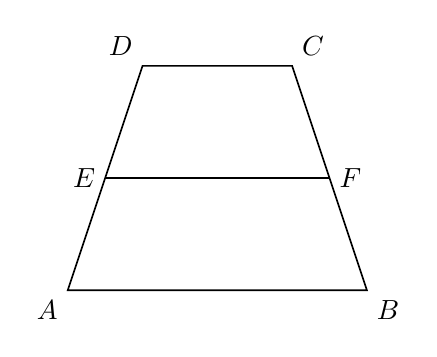
\begin{tikzpicture}[scale=0.95, >=stealth, semithick]
  % 梯形 ABCD：AB=4（下底）、CD=2（上底）、高 3；EF 为中位线 EF=3
  \draw (0,0) -- (4,0) -- (3,3) -- (1,3) -- cycle;
  \draw (0.5,1.5) -- (3.5,1.5);
  \node[below left] at (0,0) {$A$};
  \node[below right] at (4,0) {$B$};
  \node[above left] at (1,3) {$D$};
  \node[above right] at (3,3) {$C$};
  \node[left] at (0.5,1.5) {$E$};
  \node[right] at (3.5,1.5) {$F$};
\end{tikzpicture}
\end{center}
\nopagebreak[4]
\Needspace{4\baselineskip}
\textbf{解析}
设梯形的高为 $h$，$EF$ 到下底 $AB$ 的距离为 $h_1$，到上底 $CD$ 的距离为 $h_2$，则 $h_1+h_2=h$。
\Needspace{5\baselineskip}
梯形内平行于底、距 $AB$ 为 $t$ 的截线，其长随 $t$ 线性变化：$t=0$ 时为 $AB=4$，$t=h$ 时为 $CD=2$，故截线长为
\nopagebreak[4]
\[
\ell(t)=4-\frac{2t}{h}.
\]
\Needspace{5\baselineskip}
由 $EF=3$ 得
\nopagebreak[4]
\[
4-\frac{2h_1}{h}=3\ \Longrightarrow\ \frac{2h_1}{h}=1\ \Longrightarrow\ h_1=h_2=\frac h2,
\]
即 $EF$ 恰是梯形的中位线（这也与中位线长 $\dfrac{4+2}{2}=3$ 一致，题目给的 $EF=3$ 正是中位线长）。
\Needspace{5\baselineskip}
于是
\nopagebreak[4]
\[
S_{ABFE}=\frac{4+3}{2}\cdot\frac h2=\frac{7h}{4},\qquad
S_{EFCD}=\frac{3+2}{2}\cdot\frac h2=\frac{5h}{4},
\]
\Needspace{5\baselineskip}
面积比为
\nopagebreak[4]
\[
S_{ABFE}:S_{EFCD}=\frac{7h}{4}:\frac{5h}{4}=7:5.
\]
二次复算：两部分之和 $\dfrac{7h}{4}+\dfrac{5h}{4}=3h$，等于梯形总面积 $\dfrac{4+2}{2}\cdot h=3h$，无遗漏。

\gkanswer{答案：$7:5$。}

\end{answer}
\begin{answer}
\gksolhead{16}{}

\textbf{题目}：

已知函数 $f(x)=2\sin\left(\dfrac13x-\dfrac{\pi}{6}\right)$，$x\in\mathbf R$。
（1） 求 $f(0)$ 的值；
（2） 设 $\alpha$，$\beta\in\left[0,\dfrac{\pi}{2}\right]$，$f\left(3\alpha+\dfrac{\pi}{2}\right)=\dfrac{10}{13}$，$f(3\beta+2\pi)=\dfrac65$，求 $\sin(\alpha+\beta)$ 的值。

\Needspace{4\baselineskip}
\textbf{解析}
把 $f$ 的解析式写成便于代入的形式：$f(x)=2\sin\left(\dfrac x3-\dfrac{\pi}{6}\right)$。

\gksubpart{(1)}
\nopagebreak[4]
\[
f(0)=2\sin\left(0-\frac{\pi}{6}\right)=2\times\left(-\frac12\right)=-1.
\]

\gksubpart{(2)}
\Needspace{5\baselineskip}
分别化简两个已知条件，注意括号内的角正好是 $\dfrac x3-\dfrac{\pi}{6}$ 的对应值：
\nopagebreak[4]
\[
f\left(3\alpha+\frac{\pi}{2}\right)=2\sin\left(\frac{3\alpha+\frac{\pi}{2}}{3}-\frac{\pi}{6}\right)
=2\sin\left(\alpha+\frac{\pi}{6}-\frac{\pi}{6}\right)=2\sin\alpha,
\]
\nopagebreak[4]
\[
f(3\beta+2\pi)=2\sin\left(\frac{3\beta+2\pi}{3}-\frac{\pi}{6}\right)
=2\sin\left(\beta+\frac{2\pi}{3}-\frac{\pi}{6}\right)=2\sin\left(\beta+\frac{\pi}{2}\right)=2\cos\beta.
\]
\Needspace{5\baselineskip}
于是
\nopagebreak[4]
\[
2\sin\alpha=\frac{10}{13}\ \Longrightarrow\ \sin\alpha=\frac{5}{13},\qquad
2\cos\beta=\frac65\ \Longrightarrow\ \cos\beta=\frac35.
\]
\Needspace{5\baselineskip}
由 $\alpha,\beta\in\left[0,\dfrac{\pi}{2}\right]$，正弦、余弦都取非负值（且 $\sin\alpha=\dfrac{5}{13}<1$、$\cos\beta=\dfrac35<1$ 都允许），故
\nopagebreak[4]
\[
\cos\alpha=\sqrt{1-\frac{25}{169}}=\frac{12}{13},\qquad
\sin\beta=\sqrt{1-\frac{9}{25}}=\frac45.
\]
\Needspace{5\baselineskip}
两角和的公式给出
\nopagebreak[4]
\[
\sin(\alpha+\beta)=\sin\alpha\cos\beta+\cos\alpha\sin\beta
=\frac{5}{13}\cdot\frac35+\frac{12}{13}\cdot\frac45
=\frac{15+48}{65}=\frac{63}{65}.
\]
二次复算：$\alpha=\arcsin\dfrac{5}{13}\approx22.62^\circ$，$\beta=\arccos\dfrac35\approx53.13^\circ$，和为 $75.75^\circ$，$\sin75.75^\circ\approx0.9692$，而 $\dfrac{63}{65}\approx0.9692$，吻合；另外直接检验 $2\sin\alpha=\dfrac{10}{13}$、$2\cos\beta=\dfrac65$ 两个条件都已用上，无遗漏。

\gkanswer{答案（1）：$-1$。}

\gkanswer{答案（2）：$\dfrac{63}{65}$。}

\end{answer}
\begin{answer}
\gksolhead{17}{}

\textbf{题目}：

在某次测验中，有 6 位同学的平均成绩为 75 分．用 $x_n$ 表示编号为 $n$（$n=1,2,\cdots,6$）的同学所得成绩，且前 5 位同学的成绩如下：

\begin{center}
\begin{tabular}{lrrrrr}
\toprule
编号 $n$ & 1 & 2 & 3 & 4 & 5 \\
\midrule
成绩 $x_n$ & 70 & 76 & 72 & 70 & 72 \\
\bottomrule
\end{tabular}
\end{center}

（1） 求第 6 位同学的成绩 $x_6$，及这 6 位同学成绩的标准差 $s$；
（2） 从前 5 位同学中，随机地选 2 位同学，求恰有 1 位同学成绩在区间 $(68,75)$ 中的概率。

\Needspace{4\baselineskip}
\textbf{解析}
记六个成绩为 $x_1,\dots,x_6$，已知 $x_1=70$、$x_2=76$、$x_3=72$、$x_4=70$、$x_5=72$，平均成绩 $\bar x=75$。

\gksubpart{(1)}
\Needspace{5\baselineskip}
六人总分为 $6\times75=450$，前五人之和为
\nopagebreak[4]
\[
70+76+72+70+72=360,
\]
\Needspace{5\baselineskip}
故
\nopagebreak[4]
\[
x_6=450-360=90.
\]
\Needspace{5\baselineskip}
标准差按 $s=\sqrt{\dfrac1n\sum(x_i-\bar x)^2}$ 计算。六个数据与 $75$ 的偏差为 $-5,\,1,\,-3,\,-5,\,-3,\,15$，平方和为
\nopagebreak[4]
\[
25+1+9+25+9+225=294,
\]
\Needspace{5\baselineskip}
故
\nopagebreak[4]
\[
s^2=\frac{294}{6}=49,\qquad s=7.
\]

\gksubpart{(2)}
前五位同学的五个成绩中，落在区间 $(68,75)$ 内的是 $70,\,72,\,70,\,72$（四人，编号 $1,3,4,5$），不在内的是 $76$（编号 $2$）。
\Needspace{5\baselineskip}
从五人中任取两人，基本事件总数为
\nopagebreak[4]
\[
\mathrm C_5^2=10,
\]
\Needspace{5\baselineskip}
每个基本事件等可能，概率都是 $\dfrac1{10}$。恰有一人成绩在 $(68,75)$ 内：成绩为 $70$ 或 $72$ 的共 $4$ 人，另一人成绩为 $76$（$1$ 人），故事件数为
\nopagebreak[4]
\[
\mathrm C_4^1\cdot\mathrm C_1^1=4\times1=4,
\]
\Needspace{5\baselineskip}
逐个累加：
\nopagebreak[4]
\[
P=4\times\frac1{10}=\frac{4}{10}=\frac25.
\]
二次复算（列举全部 $10$ 个基本事件）：$\{1,2\}$（$70,76$，符合）、$\{1,3\}$（$70,72$，不符合）、$\{1,4\}$（$70,70$，不符合）、$\{1,5\}$（$70,72$，不符合）、$\{2,3\}$（$76,72$，符合）、$\{2,4\}$（$76,70$，符合）、$\{2,5\}$（$76,72$，符合）、$\{3,4\}$（$72,70$，不符合）、$\{3,5\}$（$72,72$，不符合）、$\{4,5\}$（$70,72$，不符合）。符合的有 $4$ 个，每个概率 $\dfrac1{10}$，合计 $\dfrac4{10}=\dfrac25$，与组合计数一致。

\gkanswer{答案（1）：$x_6=90$，$s=7$。}

\gkanswer{答案（2）：$\dfrac25$。}

\end{answer}
\begin{answer}
\gksolhead{18}{}

\textbf{题目}：

如图所示的几何体是将高为 2，底面半径为 1 的直圆柱沿过轴的平面切开后，将其中一半沿切面向右水平平移后得到的．$A$，$A'$，$B$，$B'$ 分别为 $\widehat{CD}$，$\widehat{C'D'}$，$\widehat{DE}$，$\widehat{D'E'}$ 的中点，$O_1$，$O_1'$，$O_2$，$O_2'$ 分别为 $CD$，$C'D'$，$DE$，$D'E'$ 的中点。
（1） 证明：$O_1'$，$A'$，$O_2$，$B$ 四点共面；
（2） 设 $G$ 为 $AA'$ 中点，延长 $A'O_1'$ 到 $H'$，使得 $O_1'H'=A'O_1'$．证明：$BO_2'\perp$ 平面 $H'B'G$。
\nopagebreak[4]
\begin{center}% 2011 年广东卷文科第 18 题：直圆柱沿过轴平面切成两半、其中一半沿切面向右平移后的几何体。
% 来源 PDF：普通高考/2011/2011广东文.pdf，SHA-256 b42cd0aaa193fefb6dcb39d1ae186d536a83fafbd4a64975deafbea5613d98ce。
% 原页：第 2 页（A3 三栏）第 1 栏中部，书页码 666。
% 重绘依据：照原页的斜二测画法——两半圆柱的切面共面并排，左半切面为矩形 CDD'C'（在后），
%   右半切面为矩形 DEE'D'（在前），左右两半的圆形面朝向相反。深度方向按原页量得
%   约为每单位 (−0.45, +0.45)（向右上为远），故顶点 A、A'、G、H'、B、B' 的位置由投影算出。
%   实线：C'C、CD、C'D'、D'E'、D'D、E'E、B'B、A'H'（过 O1'）、O2'B'、H'B'；
%   虚线：DE、AA'（过 G）、O2'B、左半底面的半圆（过 A）。
%   原页另在 H'B' 下方画一条由 H' 到 B' 的向下微凹虚线弧，与题设构造无关，本库照原页重绘、不赋几何含义。
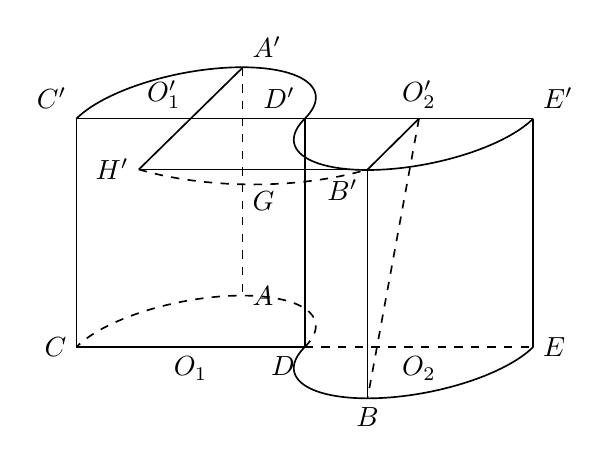
\begin{tikzpicture}[scale=1.45, >=stealth, semithick]
  % 半圆（斜二测投影后的椭圆弧）：左半上、下两弧向左上鼓出，右半两弧向右下鼓出
  \draw plot[domain=0:180, samples=90, smooth]
    ({1+cos(\x)+0.45*sin(\x)}, {2+0.45*sin(\x)});      % 左半顶面，过 A'
  \draw[dashed] plot[domain=0:180, samples=90, smooth]
    ({1+cos(\x)+0.45*sin(\x)}, {0.45*sin(\x)});        % 左半底面，不可见，过 A
  \draw plot[domain=0:180, samples=90, smooth]
    ({3+cos(\x)-0.45*sin(\x)}, {2-0.45*sin(\x)});      % 右半顶面，过 B'
  \draw plot[domain=0:180, samples=90, smooth]
    ({3+cos(\x)-0.45*sin(\x)}, {-0.45*sin(\x)});       % 右半底面，过 B
  % 切面边与可见棱
  \draw (0,2) -- (0,0) -- (2,0);                        % C'C、CD
  \draw (0,2) -- (4,2);                                 % C'D'E'
  \draw (2,2) -- (2,0);                                 % D'D
  \draw (4,2) -- (4,0);                                 % E'E
  \draw (2.55,1.5545) -- (2.55,-0.4455);                % B'B
  % 左半顶面上的半径 A'O1' 及其延长到 H'
  \draw (1.454,2.4455) -- (0.546,1.5545);               % A'H'，过 O1'(1,2)
  % 右半顶面上的半径 O2'B' 可见，O2'B 藏在体内
  \draw (3,2) -- (2.55,1.5545);                         % O2'B'
  \draw[dashed] (3,2) -- (2.55,-0.4455);                % O2'B
  % AA'（含中点 G）不可见；DE 不可见
  \draw[dashed] (1.454,2.4455) -- (1.454,0.4455);       % A'A，过 G(1.454,1.4455)
  \draw[dashed] (2,0) -- (4,0);                         % DE
  % H'B' 实线；其下的微凹虚线弧照原页保留
  \draw (0.546,1.5545) -- (2.55,1.5545);
  \draw[dashed] (0.546,1.5545) .. controls (1.15,1.38) and (1.95,1.38) .. (2.55,1.5545);
  % 顶点与中点标注
  \node[above left]  at (0,2)   {$C'$};
  \node[left]        at (0,0)   {$C$};
  \node[above left]  at (2,2)   {$D'$};
  \node[below left]  at (2,0)   {$D$};
  \node[above right] at (4,2)   {$E'$};
  \node[right]       at (4,0)   {$E$};
  \node[above right] at (1.454,2.4455) {$A'$};
  \node[right]       at (1.454,0.4455) {$A$};
  \node[below left]  at (2.55,1.5545)  {$B'$};
  \node[below]       at (2.55,-0.4455) {$B$};
  \node[left]        at (0.546,1.5545) {$H'$};
  \node[below right] at (1.454,1.4455) {$G$};
  \node[below]       at (1,0)   {$O_1$};
  \node[above left]  at (1,2)   {$O_1'$};
  \node[below]       at (3,0)   {$O_2$};
  \node[above]       at (3,2)   {$O_2'$};
\end{tikzpicture}
\end{center}
\nopagebreak[4]
\Needspace{4\baselineskip}
\textbf{解析}
\Needspace{5\baselineskip}
按原页图形的相对位置取坐标系：切面为 $y=0$ 平面（$x$ 轴水平向右、$z$ 轴竖直向上），左半圆柱的轴为 $z$ 轴，右半圆柱沿 $x$ 轴正方向平移一个直径（$2$）。圆柱高 $2$、底面半径 $1$，故
\nopagebreak[4]
\[
C(-1,0,0),\ D(1,0,0),\ E(3,0,0),\qquad
C'(-1,0,2),\ D'(1,0,2),\ E'(3,0,2),
\]
\nopagebreak[4]
\[
O_1(0,0,0),\ O_1'(0,0,2),\ O_2(2,0,0),\ O_2'(2,0,2).
\]
\Needspace{5\baselineskip}
两半圆柱的圆形面朝向相反：左半的弧鼓向 $y>0$ 一侧（$CD$ 的中点 $O_1$ 是圆心，圆弧在 $xOz$ 平面之外），右半的弧鼓向 $y<0$ 一侧。按题设「$A$、$A'$、$B$、$B'$ 分别为 $\widehat{CD}$、$\widehat{C'D'}$、$\widehat{DE}$、$\widehat{D'E'}$ 的中点」，四个中点分别是各自半圆弧的最高点，故
\nopagebreak[4]
\[
A(0,1,0),\quad A'(0,1,2),\quad B(2,-1,0),\quad B'(2,-1,2).
\]
\Needspace{5\baselineskip}
$G$ 为 $AA'$ 的中点，故 $G(0,1,1)$。$H'$ 在直线 $A'O_1'$ 上且 $O_1'H'=A'O_1'$，即 $O_1'$ 是 $A'H'$ 的中点（原页图形中 $H'$ 在 $O_1'$ 的另一侧），故
\nopagebreak[4]
\[
H'=2O_1'-A'=(0,0,4)-(0,1,2)=(0,-1,2).
\]

\gksubpart{(1)}
\nopagebreak[4]
\[
\overrightarrow{O_1'A'}=(0,1,0),\qquad \overrightarrow{O_2B}=(2,-1,0)-(2,0,0)=(0,-1,0).
\]
两者互为相反向量，故 $O_1'A'\parallel O_2B$。两条平行直线确定一个平面，因此 $O_1'$、$A'$、$O_2$、$B$ 四点共面（它们都在过 $O_1'A'$ 且平行于 $O_2B$ 的那个平面内）。
二次复算（平面方程）：由 $O_1'(0,0,2)$、$A'(0,1,2)$、$B(2,-1,0)$ 求平面，法向量可取 $\overrightarrow{O_1'A'}\times\overrightarrow{O_1'B}=(0,1,0)\times(2,-1,-2)=(1\cdot(-2)-0\cdot(-1),\ 0\cdot2-0\cdot(-2),\ 0\cdot(-1)-1\cdot2)=(-2,0,-2)$，平面为 $x+z=2$。代入 $O_2(2,0,0)$：$2+0=2$，满足，确在平面内。

\gksubpart{(2)}
\Needspace{5\baselineskip}
要证 $BO_2'\perp$ 平面 $H'B'G$，只需证 $\overrightarrow{BO_2'}$ 垂直于该平面内两条相交直线。算出三个向量：
\nopagebreak[4]
\[
\overrightarrow{BO_2'}=(2,0,2)-(2,-1,0)=(0,1,2),
\]
\nopagebreak[4]
\[
\overrightarrow{H'B'}=(2,-1,2)-(0,-1,2)=(2,0,0),\qquad
\overrightarrow{H'G}=(0,1,1)-(0,-1,2)=(0,2,-1).
\]
\Needspace{5\baselineskip}
内积：
\nopagebreak[4]
\[
\overrightarrow{BO_2'}\cdot\overrightarrow{H'B'}=0\cdot2+1\cdot0+2\cdot0=0,
\]
\nopagebreak[4]
\[
\overrightarrow{BO_2'}\cdot\overrightarrow{H'G}=0\cdot0+1\cdot2+2\cdot(-1)=2-2=0.
\]
故 $BO_2'\perp H'B'$、$BO_2'\perp H'G$。$H'B'$ 与 $H'G$ 是平面 $H'B'G$ 内过同一点 $H'$ 的两条相交直线（$\overrightarrow{H'B'}=(2,0,0)$ 与 $\overrightarrow{H'G}=(0,2,-1)$ 不共线），由线面垂直的判定定理得 $BO_2'\perp$ 平面 $H'B'G$。
二次复算（求平面法向量）：$\overrightarrow{H'B'}\times\overrightarrow{H'G}=(2,0,0)\times(0,2,-1)=(0\cdot(-1)-0\cdot2,\ 0\cdot0-2\cdot(-1),\ 2\cdot2-0\cdot0)=(0,2,4)$，与 $\overrightarrow{BO_2'}=(0,1,2)$ 成比例（$2$ 倍），说明 $BO_2'$ 正是该平面的法线方向，结论一致。

\gkanswer{答案（1）：证明见解析。}

\gkanswer{答案（2）：证明见解析。}

\end{answer}
\begin{answer}
\gksolhead{19}{}

\textbf{题目}：

设 $a>0$，讨论函数 $f(x)=\ln x+a(1-a)x^2-2(1-a)x$ 的单调性。

\Needspace{4\baselineskip}
\textbf{解析}
\Needspace{5\baselineskip}
定义域为 $(0,+\infty)$。求导：
\nopagebreak[4]
\[
f'(x)=\frac1x+2a(1-a)x-2(1-a)
=\frac{1+2a(1-a)x^2-2(1-a)x}{x}.
\]
\Needspace{5\baselineskip}
分母 $x>0$，故 $f'$ 的符号由分子
\nopagebreak[4]
\[
h(x)=2a(1-a)x^2-2(1-a)x+1
\]
决定。按 $a$ 的取值分情形讨论（题设 $a>0$）。
\textbf{情形一：$a=1$。} 此时 $h(x)\equiv1>0$，$f'(x)>0$，$f$ 在 $(0,+\infty)$ 上单调递增。
\Needspace{5\baselineskip}
\textbf{情形二：$0<a<1$。} $h$ 是开口向上的二次函数，判别式
\nopagebreak[4]
\[
\Delta=4(1-a)^2-8a(1-a)=4(1-a)\big[(1-a)-2a\big]=4(1-a)(1-3a).
\]
\begin{itemize}
\item 当 $0<a<\dfrac13$ 时 $\Delta>0$，$h$ 有两个正根（两根之和 $\dfrac{2(1-a)}{2a(1-a)}=\dfrac1a>0$、两根之积 $\dfrac{1}{2a(1-a)}>0$，故同为正）：
\end{itemize}
\nopagebreak[4]
\[
x_1=\frac{2(1-a)-\sqrt{\Delta}}{4a(1-a)}=\frac{1-\sqrt{\dfrac{1-3a}{1-a}}}{2a},\qquad
x_2=\frac{1+\sqrt{\dfrac{1-3a}{1-a}}}{2a},
\]
$h$ 在 $(0,x_1)$ 为正、在 $(x_1,x_2)$ 为负、在 $(x_2,+\infty)$ 为正，故 $f$ 在 $(0,x_1)$ 与 $(x_2,+\infty)$ 上递增，在 $(x_1,x_2)$ 上递减；
\begin{itemize}
\item 当 $\dfrac13\leqslant a<1$ 时 $\Delta\leqslant0$，$h\geqslant0$（$a=\dfrac13$ 时 $h$ 是完全平方，仅一点为零），$f$ 在 $(0,+\infty)$ 上递增。
\end{itemize}
\Needspace{5\baselineskip}
\textbf{情形三：$a>1$。} 此时 $1-a<0$，$h$ 开口向下，判别式 $\Delta=4(1-a)(1-3a)=4(a-1)(3a-1)>0$，两根之积 $\dfrac{1}{2a(1-a)}<0$，故两根异号，只有正根
\nopagebreak[4]
\[
x_3=\frac{1+\sqrt{\dfrac{3a-1}{a-1}}}{2a}
\]
（另一根 $\dfrac{1-\sqrt{\frac{3a-1}{a-1}}}{2a}<0$ 不在定义域内）。$h$ 在 $(0,x_3)$ 为正、在 $(x_3,+\infty)$ 为负，故 $f$ 在 $(0,x_3)$ 上递增，在 $(x_3,+\infty)$ 上递减。
二次复算（三点检验）：
\begin{itemize}
\item $a=\dfrac13$：$h(x)=\dfrac49x^2-\dfrac43x+1=\left(\dfrac{2x}{3}-1\right)^2\geqslant0$，仅 $x=\dfrac32$ 处为零，$f$ 严格递增，与情形二的结论一致（临界值 $\dfrac13$ 可取）；
\item $a=\dfrac12$：$\dfrac{1-3a}{1-a}=\dfrac{-1/2}{1/2}=-1<0$，此时 $\Delta=4\cdot\dfrac12\cdot\left(-\dfrac12\right)=-1<0$，$h>0$，$f$ 递增，符合「$\dfrac13\leqslant a<1$ 时递增」；
\item $a=\dfrac16$：$\dfrac{1-3a}{1-a}=\dfrac{1/2}{5/6}=\dfrac35$，$x_1=\dfrac{1-\sqrt{3/5}}{1/3}\approx0.68$、$x_2=\dfrac{1+\sqrt{3/5}}{1/3}\approx5.32$，$h$ 在两者之间为负，$f$ 先增后减再增，与「$0<a<\dfrac13$ 时有两根」的结论一致；
\item $a=2$：$x_3=\dfrac{1+\sqrt{5/1}}{4}=\dfrac{1+\sqrt5}{4}\approx0.809$，$f$ 在 $(0,0.809)$ 上递增、之后递减，与情形三一致。
\end{itemize}

\gkanswer{答案：记 $x_{1,2}=\dfrac{1\mp\sqrt{(1-3a)/(1-a)}}{2a}$。$0<a<\dfrac13$ 时 $f$ 在 $(0,x_1)$、$(x_2,+\infty)$ 上递增，在 $(x_1,x_2)$ 上递减；$\dfrac13\leqslant a\leqslant1$ 时 $f$ 在 $(0,+\infty)$ 上递增；$a>1$ 时记 $x_3=\dfrac{1+\sqrt{(3a-1)/(a-1)}}{2a}$，$f$ 在 $(0,x_3)$ 上递增、在 $(x_3,+\infty)$ 上递减。}

\end{answer}
\begin{answer}
\gksolhead{20}{}

\textbf{题目}：

设 $b>0$，数列 $\{a_n\}$ 满足 $a_1=b$，$a_n=\dfrac{nba_{n-1}}{a_{n-1}+n-1}$（$n\geqslant2$）。
（1） 求数列 $\{a_n\}$ 的通项公式；
（2） 证明：对于一切正整数 $n$，$2a_n\leqslant b^{n+1}+1$。

\Needspace{4\baselineskip}
\textbf{解析}
\Needspace{5\baselineskip}
递推式里 $a_n$ 出现在分母，先取倒数把它化成一次关系：
\nopagebreak[4]
\[
\frac{1}{a_n}=\frac{a_{n-1}+n-1}{nba_{n-1}}=\frac{a_{n-1}}{nba_{n-1}}+\frac{n-1}{nba_{n-1}}=\frac{1}{nb}+\frac{n-1}{nb}\cdot\frac{1}{a_{n-1}}\qquad(n\geqslant2).
\]
记 $c_n=\dfrac{1}{a_n}$，则 $c_n=\dfrac1{nb}+\dfrac{n-1}{nb}c_{n-1}$，且 $c_1=\dfrac1b$。

\gksubpart{(1)}
\Needspace{5\baselineskip}
猜测
\nopagebreak[4]
\[
c_n=\frac{b^{n-1}+b^{n-2}+\cdots+b+1}{nb^n}.
\]
\Needspace{5\baselineskip}
用数学归纳法证明。$n=1$ 时右端为 $\dfrac{1}{b}$，等于 $c_1$。设对 $n-1$ 成立，即 $c_{n-1}=\dfrac{b^{n-2}+b^{n-3}+\cdots+b+1}{(n-1)b^{n-1}}$，则
\nopagebreak[4]
\[
c_n=\frac{1}{nb}+\frac{n-1}{nb}\cdot\frac{b^{n-2}+\cdots+b+1}{(n-1)b^{n-1}}
=\frac{1}{nb}+\frac{b^{n-2}+\cdots+b+1}{nb^{n}}
=\frac{b^{n-1}+b^{n-2}+\cdots+b+1}{nb^{n}},
\]
\Needspace{5\baselineskip}
归纳完成。故
\nopagebreak[4]
\[
a_n=\frac{1}{c_n}=\frac{nb^n}{b^{n-1}+b^{n-2}+\cdots+b+1}.
\]
代回验证：$n=2$ 时公式给出 $a_2=\dfrac{2b^2}{b+1}$，而递推式直接算出 $a_2=\dfrac{2b\cdot a_1}{a_1+1}=\dfrac{2b^2}{b+1}$，一致；$n=3$ 时公式给出 $\dfrac{3b^3}{b^2+b+1}$，递推式给出 $a_3=\dfrac{3ba_2}{a_2+2}=\dfrac{3b\cdot\frac{2b^2}{b+1}}{\frac{2b^2}{b+1}+2}=\dfrac{6b^3}{2b^2+2b+2}=\dfrac{3b^3}{b^2+b+1}$，也一致。

\gksubpart{(2)}
\Needspace{5\baselineskip}
要证 $2a_n\leqslant b^{n+1}+1$，即
\nopagebreak[4]
\[
\frac{2nb^n}{b^{n-1}+b^{n-2}+\cdots+b+1}\leqslant b^{n+1}+1.
\]
\Needspace{5\baselineskip}
分母为正，两边同乘分母，等价于
\nopagebreak[4]
\[
2nb^n\leqslant\left(b^{n+1}+1\right)\left(b^{n-1}+b^{n-2}+\cdots+b+1\right).
\]
\Needspace{5\baselineskip}
由二元均值不等式，对正数 $b^{n+1}$ 与 $1$：
\nopagebreak[4]
\[
b^{n+1}+1\geqslant2\sqrt{b^{n+1}\cdot1}=2b^{\frac{n+1}{2}},
\]
\Needspace{5\baselineskip}
等号当且仅当 $b^{n+1}=1$，即 $b=1$。又 $b^{n-1},b^{n-2},\dots,b,1$（共 $n$ 个正数）的几何平均为
\nopagebreak[4]
\[
\left(b^{n-1}\cdot b^{n-2}\cdots b\cdot1\right)^{\frac1n}=b^{\frac{(n-1)+(n-2)+\cdots+1+0}{n}}=b^{\frac{n-1}{2}},
\]
\Needspace{5\baselineskip}
故
\nopagebreak[4]
\[
b^{n-1}+b^{n-2}+\cdots+b+1\geqslant n\,b^{\frac{n-1}{2}},
\]
\Needspace{5\baselineskip}
等号当且仅当 $b=1$。两个不等式相乘（各因子为正）：
\nopagebreak[4]
\[
\left(b^{n+1}+1\right)\left(b^{n-1}+\cdots+b+1\right)\geqslant2b^{\frac{n+1}{2}}\cdot n\,b^{\frac{n-1}{2}}=2nb^n,
\]
即 $2a_n\leqslant b^{n+1}+1$，等号当且仅当 $b=1$。
二次复算：$n=1$ 时结论为 $2b\leqslant b^2+1$，即 $(b-1)^2\geqslant0$，成立；$n=2$ 时结论为 $\dfrac{4b^2}{b+1}\leqslant b^3+1=(b+1)(b^2-b+1)$，即 $4b^2\leqslant(b+1)^2(b^2-b+1)$，取 $b=2$ 验证：左 $16$、右 $9\times3=27$，成立。

\gkanswer{答案（1）：$a_n=\dfrac{nb^n}{b^{n-1}+b^{n-2}+\cdots+b+1}$。}

\gkanswer{答案（2）：证明见解析。}

\end{answer}
\begin{answer}
\gksolhead{21}{}

\textbf{题目}：

在平面直角坐标系 $xOy$ 中，直线 $l:x=-2$ 交 $x$ 轴于点 $A$．设 $P$ 是 $l$ 上一点，$M$ 是线段 $OP$ 的垂直平分线上一点，且满足 $\angle MPO=\angle AOP$。
（1） 当点 $P$ 在 $l$ 上运动时，求点 $M$ 的轨迹 $E$ 的方程；
（2） 已知 $T(1,-1)$，设 $H$ 是 $E$ 上动点，求 $|HO|+|HT|$ 的最小值，并给出此时点 $H$ 的坐标；
（3） 过点 $T(1,-1)$ 且不平行于 $y$ 轴的直线 $l_1$ 与轨迹 $E$ 有且只有两个不同的交点，求直线 $l_1$ 的斜率 $k$ 的取值范围。

\Needspace{4\baselineskip}
\textbf{解析}
设 $M(x,y)$，$P(-2,t)$，其中 $t$ 为参数（$P$ 在直线 $l:x=-2$ 上）。题设的两个条件要一起用。

\gksubpart{(1)}
\Needspace{5\baselineskip}
「$M$ 在线段 $OP$ 的垂直平分线上」等价于 $|MO|=|MP|$：
\nopagebreak[4]
\[
x^2+y^2=(x+2)^2+(y-t)^2\ \Longrightarrow\ 4x+4+t^2-2ty=0\ \Longrightarrow\ 2ty=4x+4+t^2.\tag{①}
\]
\Needspace{5\baselineskip}
由 $|MO|=|MP|$ 知 $\triangle OMP$ 是以 $O$、$P$ 为底边端点的等腰三角形，两底角相等，故 $\angle MPO=\angle MOP$；与题设 $\angle MPO=\angle AOP$ 比较得
\nopagebreak[4]
\[
\angle MOP=\angle AOP,
\]
\Needspace{5\baselineskip}
即射线 $OM$ 与直线 $OP$ 的夹角等于射线 $OA$ 与 $OP$ 的夹角。除去 $OM$ 与 $OA$ 重合这一支（另论于后），$OM$ 必是 $OA$ 关于直线 $OP$ 的对称方向。设 $\boldsymbol e=\dfrac{1}{\sqrt{t^2+4}}(-2,t)$ 为 $OP$ 方向的单位向量，则 $\overrightarrow{OA}=(-1,0)$ 关于 $OP$ 的对称向量为
\nopagebreak[4]
\[
\boldsymbol u=2\left(\overrightarrow{OA}\cdot\boldsymbol e\right)\boldsymbol e-\overrightarrow{OA}
=2\cdot\frac{2}{\sqrt{t^2+4}}\cdot\frac{(-2,t)}{\sqrt{t^2+4}}-(-1,0)
=\left(\frac{t^2-4}{t^2+4},\ \frac{4t}{t^2+4}\right),
\]
\Needspace{5\baselineskip}
它是单位向量（$(t^2-4)^2+16t^2=(t^2+4)^2$）。故可设
\nopagebreak[4]
\[
(x,y)=s\boldsymbol u=s\left(\frac{t^2-4}{t^2+4},\ \frac{4t}{t^2+4}\right),\qquad s=|OM|>0.
\]
\Needspace{5\baselineskip}
代入 ①：
\nopagebreak[4]
\[
2t\cdot\frac{4st}{t^2+4}=4\cdot\frac{s(t^2-4)}{t^2+4}+4+t^2
\ \Longrightarrow\ \frac{8st^2}{t^2+4}=\frac{4s(t^2-4)+4(t^2+4)+t^2(t^2+4)}{t^2+4}.
\]
\Needspace{5\baselineskip}
两边乘 $t^2+4$ 并整理：
\nopagebreak[4]
\[
8st^2=4st^2-16s+t^4+8t^2+16\ \Longrightarrow\ 4s\left(t^2+4\right)=\left(t^2+4\right)^2\ \Longrightarrow\ s=\frac{t^2+4}{4}.
\]
\Needspace{5\baselineskip}
于是
\nopagebreak[4]
\[
x=\frac{t^2-4}{4},\qquad y=\frac{t^2+4}{4}\cdot\frac{4t}{t^2+4}=t.
\]
\Needspace{5\baselineskip}
消去 $t$：由 $y=t$ 得 $x=\dfrac{y^2-4}{4}$，即
\nopagebreak[4]
\[
y^2=4(x+1).
\]
这是一条开口向右、顶点为 $(-1,0)$ 的抛物线。
二次复算（取具体点验证）：取 $t=2$，则 $P(-2,2)$，$s=\dfrac{4+4}{4}=2$，$M=\left(\dfrac{0}{8},\dfrac{8}{8}\right)\cdot2=(0,2)$；检验 $|MO|=2$、$|MP|=\sqrt{4+0}=2$，等号成立；$\angle MPO$：$\overrightarrow{PM}=(2,0)$、$\overrightarrow{PO}=(2,-2)$，夹角 $45^\circ$；$\angle AOP$：$\overrightarrow{OA}=(-1,0)$、$\overrightarrow{OP}=(-2,2)$，夹角 $45^\circ$，相等。而 $(0,2)$ 满足 $y^2=4(x+1)$（$4=4$）。
\Needspace{5\baselineskip}
另需说明题面未排除的一族退化位置：若取射线 $OM$ 与射线 $OA$ 重合（$M$ 在 $x$ 轴负半轴，$M=(-s,0)$，$s>0$），则 $\angle MOP=\angle AOP$ 自动成立，$\angle MPO=\angle MOP$ 也由 $|MO|=|MP|$ 自动成立，故 $\angle MPO=\angle AOP$ 成立。由 $|MO|=|MP|$ 得 $s^2=(2-s)^2+t^2$，即 $s=\dfrac{t^2+4}{4}$，于是这一族点为
\nopagebreak[4]
\[
M\left(-\frac{t^2+4}{4},\,0\right),\qquad t\in\mathbf R,
\]
即 $x$ 轴上 $x\leqslant-1$ 的整条射线（$t=0$ 时恰为抛物线的顶点 $A(-1,0)$）。题面没有排除它，通行答案只取抛物线；本库按通行处理，把轨迹记为 $y^2=4(x+1)$，并把这条射线作为【源疑点】记录。

\gksubpart{(2)}
\Needspace{5\baselineskip}
对 $E$ 上的点 $H(x,y)$，由 $y^2=4(x+1)$ 得 $x=\dfrac{y^2}{4}-1\geqslant-1$，于是
\nopagebreak[4]
\[
|HO|=\sqrt{x^2+y^2}=\sqrt{x^2+4x+4}=\sqrt{(x+2)^2}=x+2,
\]
\Needspace{5\baselineskip}
最后一步用了 $x\geqslant-1>-2$。这恰是 $H$ 到直线 $l:x=-2$ 的距离。因此
\nopagebreak[4]
\[
|HO|+|HT|=\operatorname{dist}(H,l)+|HT|\geqslant\operatorname{dist}(T,l),
\]
因为折线 $T\to H\to$（$l$ 上的垂足）的长度不小于 $T$ 到 $l$ 的垂线段长度。$\operatorname{dist}(T,l)=1-(-2)=3$，故最小值为 $3$。
\Needspace{5\baselineskip}
等号成立要求 $H$ 落在 $T$ 向 $l$ 所作垂线段上，即 $y_H=-1$；代入轨迹方程
\nopagebreak[4]
\[
1=4(x+1)\ \Longrightarrow\ x=-\frac34,
\]
故此时 $H\left(-\dfrac34,-1\right)$，确在 $E$ 上且位于 $T(1,-1)$ 与 $l$ 之间。
\Needspace{5\baselineskip}
二次复算（直接算函数值）：沿 $E$ 取参数 $y$，$x=\dfrac{y^2}{4}-1$，
\nopagebreak[4]
\[
g(y)=|HO|+|HT|=\left(\frac{y^2}{4}+1\right)+\sqrt{\left(\frac{y^2}{4}-2\right)^2+(y+1)^2}.
\]
在 $y=-1$ 处，第一项为 $\dfrac54$，第二项被开方式为 $\left(\dfrac14-2\right)^2+0=\dfrac{49}{16}$，故 $g(-1)=\dfrac54+\dfrac74=3$。再取 $y=-3$：第一项 $\dfrac94+1=\dfrac{13}{4}$，第二项 $\sqrt{\left(\dfrac94-2\right)^2+4}=\sqrt{\dfrac1{16}+4}=\dfrac{\sqrt{65}}{4}$，$g(-3)=\dfrac{13+\sqrt{65}}{4}\approx5.27>3$；取 $y=1$：第一项 $\dfrac54$，第二项 $\sqrt{\left(\dfrac14-2\right)^2+4}=\sqrt{\dfrac{49}{16}+4}=\dfrac{\sqrt{113}}{4}$，$g(1)=\dfrac{5+\sqrt{113}}{4}\approx3.91>3$。与最小值为 $3$ 一致。

\gksubpart{(3)}
\Needspace{5\baselineskip}
过 $T(1,-1)$ 且不平行于 $y$ 轴的直线为
\nopagebreak[4]
\[
l_1:\ y+1=k(x-1),
\]
\Needspace{5\baselineskip}
斜率 $k$ 存在。把它与 $x=\dfrac{y^2}{4}-1$ 联立（用 $y$ 作变量更方便）：
\nopagebreak[4]
\[
y+1=k\left(\frac{y^2}{4}-1-1\right)=k\left(\frac{y^2}{4}-2\right)
\ \Longrightarrow\ ky^2-4y-8k-4=0.\tag{②}
\]
\begin{itemize}
\item 若 $k=0$，② 退化为 $-4y-4=0$，只有 $y=-1$ 一个解，直线 $y=-1$ 与抛物线只有一个交点，不合题意；
\item 若 $k\neq0$，② 是二次方程，判别式
\end{itemize}
\nopagebreak[4]
\[
\Delta=16+4k(8k+4)=16+32k^2+16k=16\left(2k^2+k+1\right).
\]
配方 $2k^2+k+1=2\left(k+\dfrac14\right)^2+\dfrac78>0$，故 $\Delta>0$ 对一切 $k\neq0$ 成立，② 有两个不同实根，对应两个不同的交点。
\Needspace{5\baselineskip}
所以 $l_1$ 与 $E$ 有且只有两个不同交点，当且仅当 $k\neq0$，即
\nopagebreak[4]
\[
k\in(-\infty,0)\cup(0,+\infty).
\]
二次复算：取 $k=1$，② 为 $y^2-4y-12=0$，$y=6$ 或 $y=-2$，对应交点 $(8,6)$ 与 $(0,-2)$，都在 $y^2=4(x+1)$ 上（$36=36$、$4=4$），且都满足 $y+1=x-1$（$7=7$、$-1=-1$），确是两点；取 $k=-\dfrac12$，② 为 $-\dfrac12y^2-4y+4-4=0$，即 $y^2+8y=0$，$y=0$ 或 $y=-8$，对应 $(-1,0)$ 与 $(15,-8)$，也是两点；取 $k=0$ 只有一个交点，与结论一致。

\gkanswer{答案（1）：$y^2=4(x+1)$。}

\gkanswer{答案（2）：最小值为 $3$，此时 $H\left(-\dfrac34,-1\right)$。}

\gkanswer{答案（3）：$k\neq0$。}

\end{answer}